\makeatletter%stellare(~/Fisica-Stellare)
\let\@starttocorig\@starttoc
\makeatother%%

\documentclass[10pt,xcolor={usenames},fleqn,mathserif,serif]{beamer}

%% colors
\definecolor{bittersweet}{rgb}{1.0, 0.44, 0.37}
\definecolor{brilliantlavender}{rgb}{0.96, 0.73, 1.0}
\definecolor{antiquefuchsia}{rgb}{0.57, 0.36, 0.51}
\definecolor{violetw}{rgb}{0.93, 0.51, 0.93}
\definecolor{Veronica}{rgb}{0.63, 0.36, 0.94}
\definecolor{atomictangerine}{rgb}{1.0, 0.6, 0.4}
\definecolor{darkgray}{rgb}{0.66, 0.66, 0.66}
\definecolor{brightcerulean}{rgb}{0.11, 0.67, 0.84}
\definecolor{cadmiumorange}{rgb}{0.93, 0.53, 0.18}
\definecolor{ochre}{rgb}{0.8, 0.47, 0.13}
\definecolor{midnightblue}{rgb}{0.1, 0.1, 0.44}
\definecolor{lemon}{rgb}{1.0, 0.97, 0.0}
\definecolor{grey}{rgb}{0.7, 0.75, 0.71}
\definecolor{amber}{rgb}{1.0, 0.75, 0.0}
\definecolor{almond}{rgb}{0.94, 0.87, 0.8}
\definecolor{bf}{RGB}{88, 86, 88}
\definecolor{bb}{RGB}{177, 177, 177}
\definecolor{keyword}{rgb}{0.25, 0.25, 0.28}
\definecolor{todo}{rgb}{0.75, 0.0, 0.2}
\definecolor{must}{rgb}{1.0, 0.31, 0.0}

%beamer setup
\usepackage{beamersetup}

%%%%%%%%%%%%%%%%%%%%%%%%%%%%%%%%%%% importa pacchetti
\usepackage{usepkg}
%%%%%%%%%%%%%%%%%%%%%%%%%%%%%%%%%%% Funzioni generali
\usepackage{functions}
%http://tex.stackexchange.com/questions/246/when-should-i-use-input-vs-include
\newcommand{\setmuskip}[2]{#1=#2\relax} %%problem usinig mu with calc (req by mathtools) loaded

\usepackage{sources}


%\usepackage{length}
%%%%%%%%%%%%%%%%%%%%%%%%%%%%%%%%%%% Funzioni per questo file main
\usepackage{mathOp}

\def\status{coazione}%ripeter
\def\keeptrying{coazione}
\usepackage{LocalF}
%%%%%%%%%%%%%%%%%%%%%%%%%%%%%%%%%

\title{Fisica stellare}

% Let's get started
\begin{document}

\begin{filecontents}{conservedvector.tex}

\centering
\begin{figure}
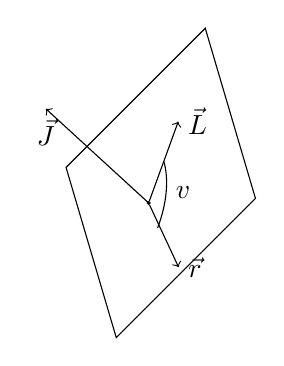
\begin{tikzpicture}[rotate around z=45, rotate around x=-45]
\draw (0,-0.3,0) -- (2.5,-0.3,0) -- (2.5,2.5,0) -- (0,2.5,0) -- cycle;
\draw[->] (1.,1.,0)node[draw,circle,inner sep=0] (o) {} -- (1.5,1.5,2)node[below] {$\vec{J}$};
\draw[->] (o) -- ++(295:0.9cm)node[right] {$\vec{r}$};
\draw[->] (o) -- ++(70:1.1cm)node[right] {$\vec{L}$}node [midway] (aux){};
\draw (aux) arc (0:-50:1) node[midway,right] {$v$};
\end{tikzpicture}

\label{fig:Lenztikz}

\end{figure}

\end{filecontents}%%contain tikz files as filecontents

\addtobeamertemplate{block begin}{\setlength\abovedisplayskip{2pt}\setlength\belowdisplayskip{2pt}\setlength\abovedisplayshortskip{2pt}\setlength\belowdisplayshortskip{2pt}}{}
\addtobeamertemplate{block begin}{\vspace*{-3pt}}{}
\addtobeamertemplate{block end}{}{\vspace*{-3pt}}

\begin{frame}
  \titlepage
\end{frame}

% Section and subsections will appear in the presentation overview
% and table of contents.
%\frame{\tableofcontents[onlyparts]}

\begin{frame}[label={argomenti}]{Fisica stellare: argomenti del corso}
    \tableofcontents[onlyparts]
\end{frame}

\begin{wordonframe}{Meta.}
lbf, todo, keyword, must
\end{wordonframe}

\begin{wordonframe}{Perch\'e studio queste cose?? Sviluppi; futuro.}

Concretezza, concentrazione, indipendenza

\end{wordonframe}

\part{Intro}\linkdest{intro}
\section{Fonti}

\begin{wordonframe}{Fisica della materia (Doni)}

\end{wordonframe}

\input{succo}

\part{Termodinamica, fisica statistica}\linkdest{thermnstat}
\begin{frame}{this part toc}
\begin{itemize}
\item (corpo nero)
\end{itemize}
\end{frame}
\section{Strumenti e situazioni in MQ}

\begin{frame}{When density of state function is a good approx to actual discrete energy states?}
If states are close enough together:
\begin{align*}
    &n_0^2=\frac{2mL^2E}{\hbar^2}=\frac{3mL^2kT}{\hbar^2}\tag{Def $n_0$ from thermal energy}\\
    &\Delta E=\frac{\hbar^2}{2mL^2}(2n_0-1)\approx\frac{h^2n_0}{mL^2}\tag{energy level separation}\\
    &T_g=\frac{\Delta E}{k}\ll T
\end{align*}
\end{frame}

\begin{frame}{Densit\'a stati particle in a box and harmonic oscillator}
    $g(E)=\TDy{E}{N}$: numero di stati tra $[E,E+dE]$ (vedi anche $g(\vec{k})$)
\begin{columns}[T]
 \begin{column}{0.5\textwidth}
\begin{align*}
    &E_{1D}=\alpha n^2=\frac{\hbar^2k_n^2}{2m}\\
    &\rho\,dk=(\Delta n_x)=\frac{L}{2\pi}\,dk\\
    &g_{1D}(E)=\frac{1}{2\alpha^{1/2}}E^{1/2},\ g(k)=\frac{L}{2\pi}\\
    &E_{3D}=\alpha n^2=(n_x^2+n_y^2+n_z^2)\alpha\\
    &N=\frac{\pi N^3}{6}\\
\end{align*}
 \end{column}
 \end{columns}
 \todo{Modification for ground state  of BE gas in low T limiti: Riedi, thermal physics, sec 10.1}
\end{frame}

\section{Bosoni}

\subsection{Fotoni}

\begin{frame}{I Fotoni}
Bosoni con $S=1$ solo traffsverso, non interagiscono tra loro (eqs. di Maxwell sono lineari): gas perfetto
\end{frame}

\begin{frame}{Corpo nero}
    Il numero di fotoni in equilibrio con pareti ta temperatura T fluttua attorno a valor medio richiesto da condizione di equilibrio. Statistica di BE con $\mu=0$ (energia interna non muta con T, V fissi, $\mu=\PDy{N}{F}$), la funzione di partizion:
\begin{align*}
    &Z(T,V)=\sum_{\{n_r\}}\exp{-\beta\sum_rn_r\epsilon_r}=\sum_{n_1=0}\ldots\sum_{n_j}=\prod_{r=1}^{\infty}\frac{1}{1-\exp{-\beta\epsilon_r}}\\
    &\exv{n_r}=-\frac{1}{\beta}\PDy{\epsilon_r}{\log{Z}|_{T,V}}=\frac{1}{\beta}\PDof{\epsilon_r}\log{(1-\exp{-\beta\epsilon_r})}=\frac{1}{\exp{\beta\epsilon_r}-1}\\
    &(\Delta n_r)^2=-\beta\PDy{\epsilon_r}{\exv{n_r}}=\exv{n_r}(1+\exv{n_r})
\end{align*}
Conta degli stati con energia con energia $\epsilon$ ($\epsilon=\hbar\omega$, $\epsilon=pc$, $p=2\pi\frac{\hbar}{\lambda}=\hbar\frac{\omega}{c}$):
\begin{align*}
    &dn_p=2 V\frac{4\pi}{h^3}p^2\,dp\tag{2 polarization}\\
    &=\frac{V8\pi}{h^3}(\frac{\hbar\omega}{c})^2\frac{\hbar\,d\omega}{c}=\frac{V}{\pi^2}\frac{\omega^2\,d\omega}{c^3}\\
    &
\end{align*}
\end{frame}



\end{document}
